
\chapter{Strategiespiele und Spieltheorie}
\label{cha:Strategiespiele und Spieltheorie}

In diesem Kapitel werden die Strategiespiele Tic Tac Toe Abschnitt \ref{sec:Das Strategiespiel Tic Tac Toe} und Reversi Abschnitt \ref{sec:Das Strategiespiel Reversi} vorgestellt und das jeweilige Regelwerk wird definiert. Weiterhin werden verschiedene Konzepte der Spieltheorie Abschnitt \ref{sec:Spieltheorie} genauer erklärt und veranschaulicht. Die \ref{subsec:Minimax} Minimax-Suche und die \ref{subsec:Alpha-Beta-Kürzung} Alpha-Beta-Kürzung sind Suchbaumverfahren die in Zweipersonenstrategiespielen eingesetzt werden. Die Alpha-Beta-Kürzung ist eine Verbesserung der Minimax-Suche und kein völlig anderes Suchverfahren. Es werden noch drei weitere Verbesserungsmöglichkeiten für die Minimax-Suche bzw. die Alpha-Beta-Suche erklärt. Die \ref{subsec:Iterativ vertiefende Tiefensuche} Iterativ vertiefende Tiefensuche ist ein Verfahren, welches Breitensuche und Tiefensuche kombiniert und bis zu einer bestimmten Suchtiefe ein bestmögliches Ergebnis sucht. Die \ref{subsec:Übergangstabellen} Übergangstabellen beschreiben eine Möglichkeit Übergänge zu vermeiden. Übergänge sind identische Spielsituationen, die von Suchbaumverfahren als unterschiedliche Spielsituationen erkannt werden und daher redundante Suchbaumzweige darstellen. Das letzte, in dieser Arbeit behandelte, Konzept der Spieltheorie, ist die Heuristik. Eine \ref{subsec:Heuristik} Heuristik ist eine Bewertungsfunktion B(s), welche für jeden Spielzustand (Stellung der Spielfiguren) s eine Schätzung bereitstellt. Die Bewertung sagt aus, wie Wertvoll ein Spielzustand s ist.

\section{Das Strategiespiel Tic Tac Toe}
\label{sec:Das Strategiespiel Tic Tac Toe}

Tic Tac Toe ist ein Spiel, welches von genau zwei Spielern gespielt wird. Während eines gesamten Spiels darf ein Spieler nur Kreuze setzen und der andere Spieler nur Kreise. Ein Spieler der während einer Partie nur Kreuze setzen darf wird als Kreuzspieler und sein Gegner als Kreisspieler bezeichnet. Wir können uns die Kreuze und Kreise als Spielsteine vorstellen, die sobald sie auf das Spielfeld gesetzt wurden, nicht mehr verändert oder verschoben werden können. Das Spielbrett ist eine 4 x 4 große Matrix, also können maximal 16 Spielsteine in diese Matrix gesetzt werden. Der Kreuzspieler muss immer als erster beginnen. Im ersten Spielzug stehen dem Kreuzspieler 16 mögliche Positionen zur Verfügung. Die Anzahl der möglichen Positionen reduziert sich jede Runde um 1, weil jede Runde genau ein gesetzter Spielstein ein Spielfeld besetzt. Folglich ist die maximale Länge einer Spielzugsequenz bei einem 4 x 4 Spielfeld gleich 16. Es ist auch möglich, dass das Spiel bereits vor der 16. Runde beendet wird. \\

\paragraph{Spielzüge} jeder Spieler setzt abwechselnd entweder ein Kreuz oder einen Kreis in ein Spielfeld des Spielbretts. Ein Spielstein kann in jedes der 16 Spielfelder gesetzt werden, außer dieses ist bereits mit einem anderen Spielstein besetzt, dann muss der Spieler ein anderes Spielfeld auswählen. Die Spieler führen solange Ihre Spielzüge aus, bis eine Siegesformation eines Spielsteintyps erreicht ist oder alle Spielfelder besetzt sind. 

\paragraph{Ziel des Spiels} ist es vier Kreuze oder vier Kreise in einer bestimmten Position anzuordnen. Es existieren mehrere unterschiedliche Anordnungen von Spielsteinen, die das Spiel beenden und einen Sieg herbeiführen. Bei einem 4 x 4 Spielfeld existieren vier vertikale, vier horizontale und zwei diagonale Anordnungen der Spielfiguren, welche einen Sieg herbeiführen würden. Insgesamt zehn verschiedene Siegesanordnungen für beide Spieler. Sind alle Spielfelder besetzt und für keinen der Spieler ist eine Siegesformation aufgetreten, dann gewinnt beziehungsweise verliert keiner der beiden Spieler und es entsteht ein Unentschieden. Gewinnt ein Spieler mit einer Siegesanordnung seiner Spielsteine, dann verliert der andere Spieler dadurch automatisch in gleicher Höhe (Nullsummenspiel). \\

\begin{figure}[!htbp]
  \centering
  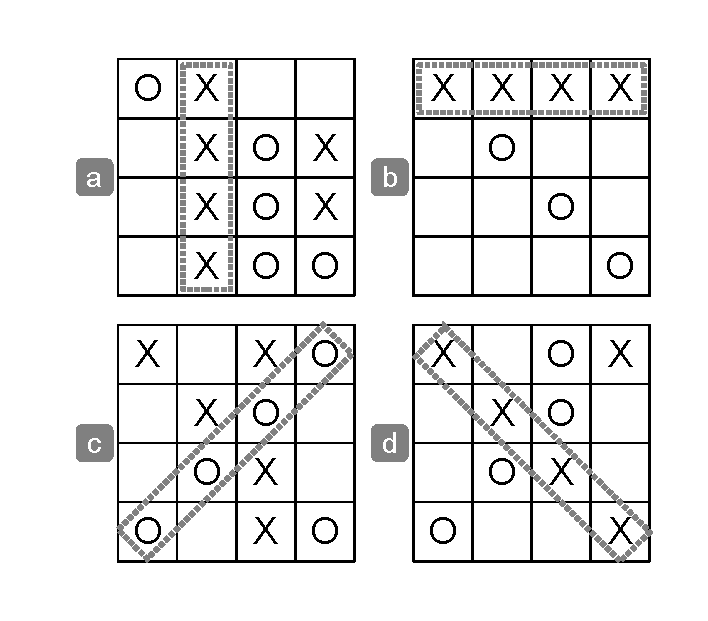
\includegraphics[scale = 0.6]{inhalt/abbildungen/siegesbedingungen_tictactoe.pdf}
  \caption{Veranschaulichtes Ziel des Strategiespiels Tic Tac Toe.}
  \label{fig:siegesbedingungen_tictactoe}
\end{figure}

Vier mögliche Siegesformationen sind in Abbildung \ref{fig:siegesbedingungen_tictactoe} dargestellt. (a) Der Kreuzspieler gewinnt knapp gegen seinen Kontrahenten mit einer ununterbrochenen vertikalen Anordnung seiner Spielsteine. Der Kreisspieler hätte fast eine diagonale Reihe aus Kreisen verbunden, diese wurde jedoch vom Kreuzspieler mit einem Spielstein unterbrochen. Zudem hätte der Kreisspieler auch fast eine vertikale Reihe ohne Unterbrechungen vervollständigt, aber der Sieg des Kreuzspielers hat die Partie vorher beendet. (b) Der Kreuzspieler erreicht eine horizontale Siegesanordnung, vier Kreuzsteine in einer horizontalen Zeile angeordnet. (c) Der Kreisspieler besiegt den Kreuzspieler mit einer diagonalen Siegesanordnung. (d) Der Kreuzspieler gewinnt ebenfalls durch eine diagonale Siegesformation seiner Spielsteine. 


\section{Das Strategiespiel Reversi}
\label{sec:Das Strategiespiel Reversi}
Das Spiel Reversi oder auch Othello genant, wird auf einem 8 x 8 Spielbrett gespielt. Es ist ein Spiel für zwei Personen die gegeneinander antreten. Eine Person setzt weiße runde Spielsteine und die andere Person schwarze runde Spielsteine. Jede neue Partie Reversie beginnt im selben Ausgangszustand (siehe Abbildung \ref{fig:ausgangssituation_reversi}). Die Spieler setzen nacheinander in ihren Spielzügen genau einen Spielstein. Wie beim klassischen Tic Tac Toe aus Abschnitt \ref{sec:Tic Tac Toe} behalten die Spieler während des gesamten Spiels ihre Spielsteinfarbe und einmal gesetzte Spielsteine können ihre Position nicht mehr verändern. \\

Anmerkung zu Abbildung \ref{fig:ausgangssituation_reversi}  Die äußeren weiß hinterlegten Reihen in denen sich Zahlen befinden, dienen dazu die Positionen der einzelnen Spielfelder genau zu definieren. In der Ausgangsspielsituation befinden sich bereits 2 weiße Spielsteine an den Positionen (3,4) und (4,3) und zwei schwarze Spielsteine an den Positionen (3,3) und (4,4). \\

\begin{figure}[!htbp]
  \centering
  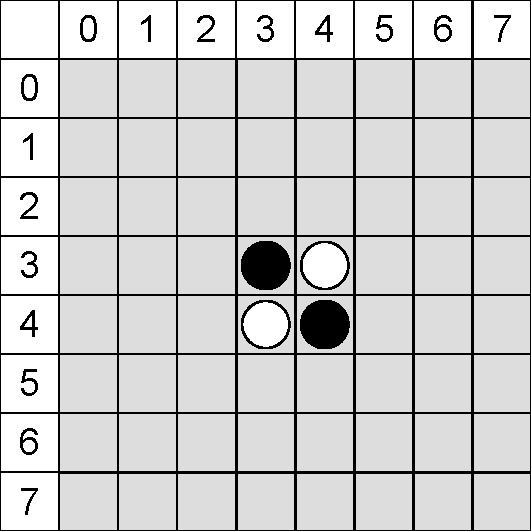
\includegraphics[scale=0.5]{inhalt/abbildungen/ausgangssituation_reversi.pdf}
  \caption{Ausgangsspielzustand Reversi.}
  \label{fig:ausgangssituation_reversi}
\end{figure}

Eine Besonderheit von Reversi ist, dass gesetzte Spielsteine ihre Farbe ändern können. Werden z.B. zwei weiße Spielsteine von zwei schwarzen in einer horizontalen Linie eingeschlossen, dann werden die weißen Spielsteine in schwarze umgewandelt beziehungsweise umgedreht. Das erobern der gegnerischen Spielsteine ist vom aktuell gesetzten Spielstein abhängig. 

\paragraph{Spielzüge} sind bei Reversi nicht beliebig, sie unterliegen bestimmten Regellungen. Eine Regel für das Setzen eines Spielsteins ist, nur wenn mindestens ein gegnerischer Spielstein erobert wird, darf ein Spielstein an diese Stelle gesetzt werden. Weiterhin  darf ein Spielstein nur dann gesetzt werden wenn, ein anderer Spielstein (Anker), mit der gleichen Farbe, in einer diagonalen, vertikalen oder horizontalen Linie, existiert. Es dürfen auch keine freien Felder zwischen dem zu setzendem Stein und dem Anker liegen. Ein Anker ist ein Spielstein mit der selben Farbe wie der zu setzende Spielstein. Ein zu setzender Spielstein kann mehrere Anker haben, aber er muss mindestens einen und kann maximal acht Anker haben.\\

\begin{figure}[!htbp]
  \centering
  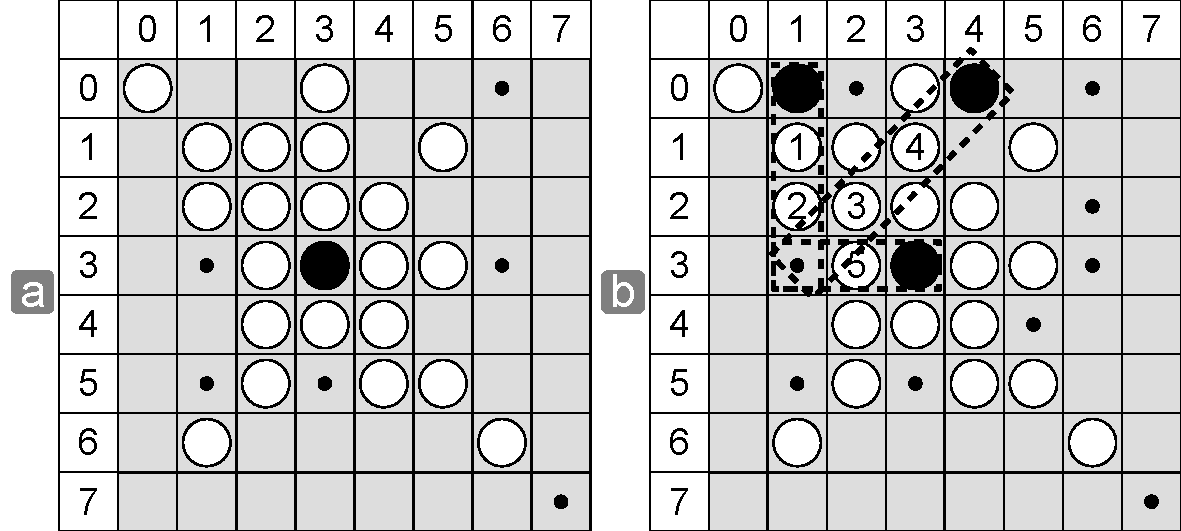
\includegraphics[scale=0.5]{inhalt/abbildungen/zuege_schwarz_reversi.pdf}
  \caption{Spielzugmöglichkeiten Reversi.}
  \label{fig:zuege_schwarz_reversi}
\end{figure}

Anmerkung zu Abbildung \ref{fig:zuege_schwarz_reversi}, diese zeigt zwei möglicherweise nicht in der Praxis auftretende Spielsituationen, die einzig verdeutlichen sollen welche Zugmöglichkeiten der Spieler mit den schwarzen Spielsteinen hat und warum nur diese Züge möglich sind. Die kleinen schwarzen Punkte zeigen die Positionen an denen ein schwarzer Spielstein gesetzt werden darf. (a) Eine Spielsituation mit maximal einem möglichen Anker. (b) Eine Spielsituation mit maximal 3 möglichen Ankern für die Position (3,1). \\

Der Anker in Abbildung \ref{fig:zuege_schwarz_reversi} (a) ist der schwarze Spielstein an der Stelle (3,3). In diesem Beispiel soll schwarz am Zug sein und einen Spielstein platzieren. Die Positionen (3,1) und (3,6) ermöglichen eine horizontale, (5,3) ermöglicht eine vertikale und (5,1), (0,6) und (7,7) ermöglichen eine diagonale Verbindung mit dem Anker auf Position (3,3). Die meisten gegnerischen Spielsteine könnte schwarz erobern, indem er seinen Spielstein auf das Spielfeld (7,7) setzt. In Abbildung \ref{fig:zuege_schwarz_reversi} (b) setzt der Spieler seinen schwarzen Spielstein an die Position (3,1), dann hat dieser 3 Anker. Einen vertikalen Anker (0,1), einen horizontalen Anker (3,3) und einen diagonalen Anker (0,4). Insgesamt würden 5 weiße Spielsteine erobert werden, also 2 mehr als in (a) maximal möglich wären. \\

\paragraph{Ziel des Spiels} ist es, am Ende des Spiels mehr Spielsteine seiner eigenen Farbe zu haben, als der Gegner Spielsteine in seiner Farbe hat. Das Spiel endet, wenn keiner der beiden Spieler mehr einen Spielstein, nach den Regeln des Spiels, auf das Spielbrett setzen kann. \\

\section{Spieltheorie}
\label{sec:Spieltheorie}
Schach, Vier Gewinnt, Dame, Tic Tac Toe und Reversi sind strategische Spiele für zwei Personen, die gegeneinander antreten, um nach den Regeln des Spiels, den Gegenspieler zu besiegen. Diese Spiele sind deterministisch weil, dass Spiel nicht vom Zufall abhängt und der gleiche Spielzug führt bei gleichem Ausgangszustand immer zum selben Zustandsübergang. Zudem sind sie überschaubar weil, zu jedem Zeitpunkt des Spiels das Spielfeld und alle Spielzüge einsehbar sind. Ein nichtdeterministisches Spiel mit Gegenspieler ist z.B. Backgammon, denn Würfelergebnisse und somit der Zufall sind Bestandteil des Spiels. Wie kann ein Programm einen Menschen in einem dieser Strategiespiele besiegen? In den nachfolgenden Unterabschnitten werden Konzepte der Spieltheorie erläutert, die versuchen diese Frage zu beantworten.

\myparagraph{Nullsummenspiele} 
Ein Nullsummenspiel ist ein Spiel bei dem der Verlust eines Spielers einen gleich hohen Gewinn für den Gegenspieler bedeutet. Gewinnt ein Spieler eine Partie eines Nullsummenspiels, dann verliert der Gegenspieler automatisch. Der gewinnende Spieler erhält einen Pluspunkt und der verlierende Spieler einen Minuspunkt. Die Summe der beiden Ergebnisse ist Null. Gewinnt beziehungsweise verliert keiner der beiden Spieler, dann erhalten beide Spieler als Spielergebnis eine Null. Die Summe der beiden Ergebnisse ist wiederum Null, so lässt sich der Name "Nullsummenspiele" herleiten. Die beiden Spiele Tic Tac Toe und Reversi sind Nullsummenspiele. 

\subsection{Minimax}
\label{subsec:Minimax}
Ein Spieler wird als MAX bezeichnet und der Gegenspieler als MIN. Spieler MAX versucht einen maximalen Gewinn für sich zu erlangen und Spieler MIN versucht den erreichbaren Gewinn von MAX zu minimieren. Es wäre auch möglich anzunehmen, dass Spieler MIN einfach irgendeinen zufälligen oder dummen Spielzug auswählt und MAX einen einfachen Sieg erlangt. Diese Annahme entspricht jedoch wenig einem realen Spiel, bei dem beide Spieler versuchen das Spiel zu gewinnen.\\

In Abbildung \ref{fig:minimax_tictactoe} ist der Ablauf einer Minimax-Suche veranschaulicht. Der Minimax-Suchbaum berücksichtigt jeden Zustand indem sich die Spielwelt befinden kann. Im ersten Spielzug könnte Spieler MAX sein Kreuzspielstein in die obere linke Ecke setzen, daraus ergeben sich neue Zustandsmöglichkeiten. Spieler MIN könnte seinen Kreisspielstein ein Feld weiter rechts und in die selbe Reihe wie Spieler MAX setzen. Der Nutzen der einzelnen Züge ist zur Zeit der Ausführung noch nicht bekannt, erste wenn das Tic Tac Toe Spiel einen Endzustand erreicht, werden den Spielern ihre Spielergebnisse mitgeteilt. Der Minmax-Suchbaum ist somit rekursiv zu betrachten. Von seinen Blattknoten ausgehend entscheidet sich MIN für den geringsten Nutzwert und MAX für den höchsten. Die Entscheidungen stehen in direkter Abhängigkeit zur vorherigen Entscheidung des Gegenspielers. \\
  
\begin{figure}[!htbp]
  \centering
  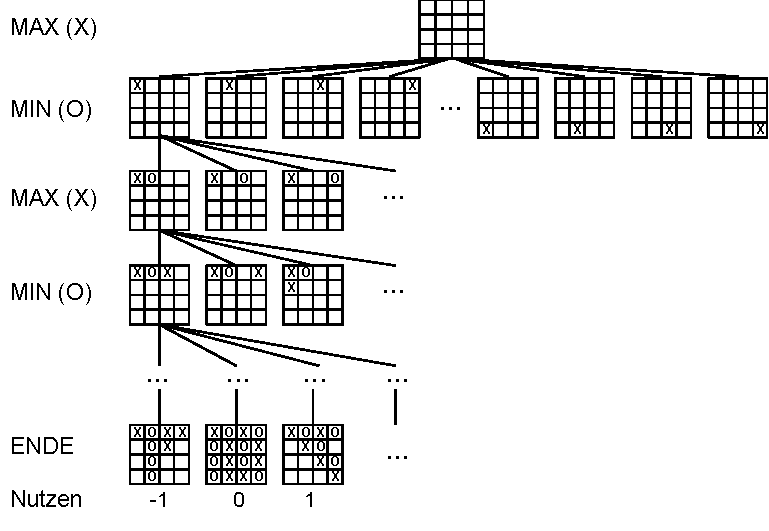
\includegraphics{inhalt/abbildungen/minimax_tictactoe.pdf}
  \caption{Ein (partieller) Suchbaum vgl. \cite[208]{Russell}}
  \label{fig:minimax_tictactoe}
\end{figure} 

Das größte Problem der Minimax-Suche ist die exponentielle Vergrößerung der Anzahl der Blattknoten des Suchbaums, schon bei sehr einfachen Spielen z.B. einem 3x3 Tic Tac Toe mit Neun Spielfeldern ist der Suchbaum bereits sehr groß ungefähr 362880 Blattknoten mit einem effektiven Verzweigungsfaktor von Neun der sich nach jedem Halbzug um Eins verringert. Erweitern wir die Dimension des Tic Tac Toe Spiels, so erhalten wir ein 4x4 Tic Tac Toe Spiel mit 16 Spielfeldern, einem Verzweigungsfaktor von 16 und ungefähr 20922789888000 Blattknoten. Der effektive Verzweigungsfaktor beim Schach liegt etwa bei 30 bis 35. Bei einem typischen Spiel mit 50 Zügen pro Spieler hat der Suchbaum dann mehr als $30^{100} \approx 10^{148}$ Blattknoten\cite[114]{Ertel}. Der Minimax-Algorithmus ist, auf Grund enormer Rechenzeit, in seiner Reinform praktisch nicht anwendbar, daher werden wir Erweiterungen der Minmax-Suche und andere Konzepte kennen lernen.

\subsection{Alpha-Beta-Kürzung}
\label{subsec:Alpha-Beta-Kürzung}
Eine Möglichkeit die Rechenzeit der Minimax-Suche zu verbessern ist das Kürzen oder Beschneiden des Suchbaums(eng. Pruning). Beim Alpha-Beta-Kürzen wird der Teil des Suchbaums beschnitten, der keinen Effekt auf das Ergebnis der Minimax Suche hat. Der Minimax Algorithmus wird um zwei Parameter Alpha und Beta ergänzt. Die Bewertung erfolgt an jedem Blattknoten des Suchbaums. Alpha enthält den aktuell größten Wert, für jeden Maximum Knoten, der bisher bei der Traversierung des Suchbaums gefunden wurde. In Beta wird für jeden Minimum Knoten der bisher kleinste gefundene Wert gespeichert. Ist Beta an einem Minimum Knoten kleiner oder gleich Alpha ($Beta \leq Alpha$), so kann die Suche unterhalb von diesem Minimum Knoten abgebrochen werden. Ist Alpha an einem Maximum Knoten größer oder gleich Beta ($Alpha \geq Beta$), so kann die Suche unterhalb von diesem Maximum Knoten abgebrochen werden \cite[116]{Ertel}. \\

\begin{figure}[!htbp]
  \centering
  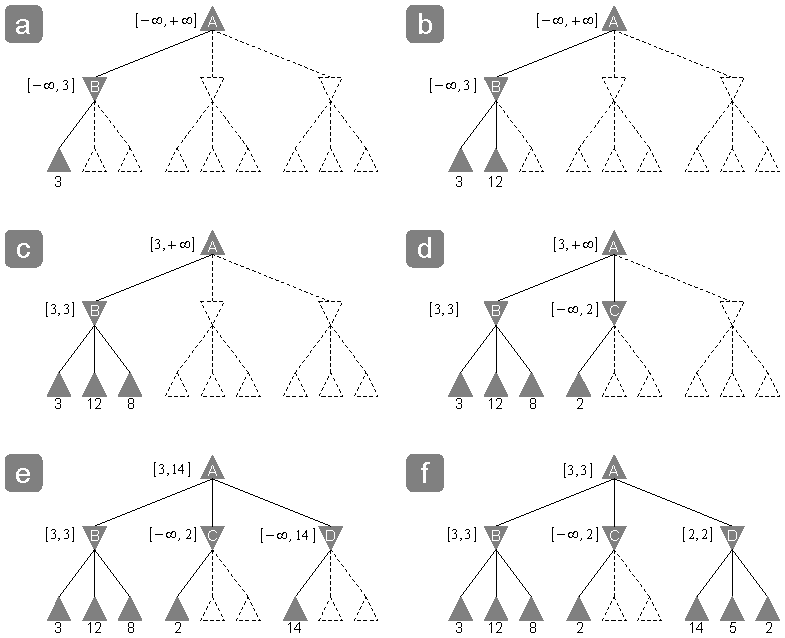
\includegraphics[scale = 0.8]{inhalt/abbildungen/alpha_beta_suchbaum.pdf}
  \caption{Ein Alpha Beta Suchbaum \cite[213]{Russell}.}
  \label{fig:minimax_tictactoe}
\end{figure} 

Verdeutlichen wir das Alpha-Beta-Pruning an Hand eines Beispiels aus dem Standardwerk der künstlichen Intelligenz von S. Russell und P. Norvig Abbildung 5.5 \cite[213]{Russell}. Ein Dreieck mit der Spitze nach oben ist ein Maximumknoten und ein Dreieck mit der Spitze nach unten ist ein Minimumknoten. Leere Dreiecke ohne einen bezeichnenden Buchstaben und gestrichelter Umrandung sind noch nicht explorierte Knoten. Durchgängige Linien verweisen auf bereits besuchte Pfade und gestrichelte Linien verweisen auf noch nicht besuchte Pfade. Die Zahlen unterhalb der Blattknoten sind die Nutzwerte die der maximierende Spieler erhält, wenn er den Pfad bis zu diesem Blattknoten durchschreitet. \\

(a) Minimum Knoten B findet einen Nutzwert 3, da dieser Wert der bisher kleinste gefundene Wert ist wird er in Beta gespeichert. \\

(b) Der Minimum Knoten B exploriert einen zweiten möglichen Nutzwert 12. Dieser Wert ist höher als der vorher gefundene und in Beta gespeicherte Wert 3, daher wird der minimierende Spieler versuchen diesen Nutzwert für den maximierenden Spieler zu vermeiden. Der neue Wert wird vom Minimum Knoten B ignoriert und Beta bleibt unverändert. \\

(c) Minimum Knoten B findet den Wert 8, dieser ist genau wie 12 größer als 3 und daher wird Spieler MIN vermeiden, dass Spieler MAX zu diesem Spielergebnis gelangt. Minimum Knoten B hat alle seine nachfolgenden Knoten exploriert. Maximum Knoten A wird vom Minimum Knoten B maximal den Nutzwert 3 erhalten, somit ergibt sich für den Maximum Knoten A, dass dieser mindestens den Nutzwert 3 erreichen kann. \\

(d) Ein weiterer Minimum Knoten ist C. Der erste Blattknoten von C liefert einen Nutzwert von 2, weil dieser Wert der erste gefundene Wert unterhalb des Minimum Knotens C ist, wird er in Beta gespeichert. C wird Maximum Knoten A maximal einen Nutzwert 2 liefern. A wiederum kann durch Minimum Knoten B bereits einen minimalen Nutzwert von 3 erhalten und hat diesen in Alpha gespeichert. Es gilt $Beta \leq Alpha$ und es ist nicht notwendig die Knoten unterhalb von C weiter zu explorieren. Selbst wenn ein größerer Nutzwert gefunden werden würde, entscheidet sich der minimierende Spieler trotzdem für den kleineren Wert und würde ein kleinerer Nutzwert als 2 gefunden werden, dann entscheidet sich der maximierende Spieler für den Nutzwert 3, den Minimum Knoten B liefert. Folglich kann der Suchbaum an dieser Stelle abgeschnitten werden, weil weitere gefundene Nutzwerte keinen Einfluss mehr auf das Ergebnis haben. \\

(e) Der letzte von A zu erreichende Minimum Knoten wird exploriert. Der erste Blattknoten unterhalb des Minimum Knoten D liefert den Nutzwert 14. Dieser Wert wäre für Maximum Knoten A eine starke Verbesserung, weil dieser bisher nur maximal einen Nutzwert von 3 erreichen konnte. Der minimierende Spieler hat noch zwei weitere Möglichkeiten(Knoten) zu explorieren und daher wird er versuchen einen geringeren Nutzwert als 14 zu finden. \\

(f) Minimum Knoten D findet in den beiden letzten Blattknoten die Nutzwerte 5 und 2. Der minimierende Spieler wählt die Möglichkeit mit dem geringsten Nutzwert 2. Dieser Nutzwert wird zum neuen Beta Wert. Der Suchbaum wird unterhalb vom Minimum Knoten D jedoch nicht abgeschnitten, weil der Nutzwert 2 erst im zuletzt explorierten Knoten gefunden wurde. Theoretisch könnten zwei Pfade unterhalb des Minimum Knoten D abgeschnitten werden, wenn der Blattknoten mit dem Nutzwert 2 zuerst exploriert worden wäre.

\subsection{Iterativ vertiefende Tiefensuche}
\label{subsec:Iterativ vertiefende Tiefensuche}
Die iterativ vertiefende Suche (eng. Iterative Deepening) ist eine Kombination der Breitensuche und der Tiefensuche. Diese Suchverfahren sind uninformierte (blinde) Suchverfahren. Die Strategien der uninformierten Suchverfahren haben keine zusätzlichen Informationen über Zustände, außer den in der Problemdefinition vorgegebenen. Alles was sie tun können, ist, Nachfolger zu erzeugen und einen Zielzustand von einem Nichtzielzustand zu unterscheiden. Die Reihenfolge der Suche ist entscheidend für die Unterscheidung der einzelnen uninformierten Suchverfahren \cite[116]{Russell}. \\
 
\begin{figure}[!htbp]
  \centering
  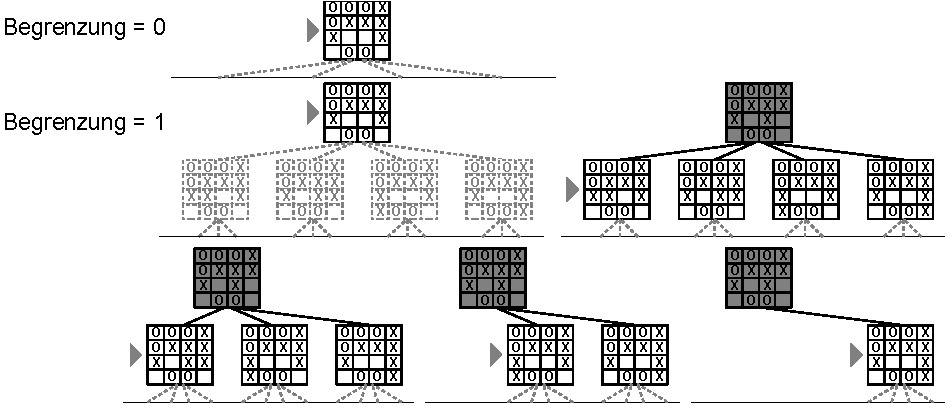
\includegraphics[scale = 0.9]{inhalt/abbildungen/iterative_deepening_tictactoe.pdf}
  \caption{TODO }
  \label{fig:minimax_tictactoe}
\end{figure}  
 
\paragraph{Die Breitensuche} expandiert (erweitert oder vergrößert) zu erst alle Nachfolger (Knoten eines Suchbaums) die in derselben Tiefe liegen, beginnend mit dem Wurzelknoten. Sind alle Nachfolger einer Tiefe expandiert, dann werden deren Nachfolger nacheinander expandiert. Diesen Schritt wiederholt die Breitensuche bis ein gesuchtes Ergebnis gefunden wird. \\

\paragraph{Die Tiefensuche} expandiert zuerst die tiefsten Knoten des Suchbaums(Depth-first). Erreicht die Tiefensuche einen Endknoten der nicht dem gesuchten Ergebnis entspricht, dann werden die alternativen Knoten des letzten expandierten Knotens, der sich eine Tiefenebene höher befindet, expandiert. \\

Kombinieren wir diese beiden uninformierten Suchverfahren miteinander und mit einer Grenze für die Suchtiefe, erhalten wir die iterative Tiefensuche. Diese expandiert zuerst die Nachfolger des Wurzelknotens der Suchtiefe 1. Sind alle Knoten auf dieser Ebene expandiert, dann wird die Schranke für die aktuelle Suchtiefe um 1 erhöht (Iteration) und die Knoten der Suchtiefe 2 werden expandiert. Diese Schritte wiederholt die Tiefensuche bis ein Ziel gefunden wird.  

\paragraph{Anwendung} findet die iterative Tiefensuche bei der Zugsortierung für die Verbesserung des Alpha-Beta Suchbaumkürzens. 


\subsection{Übergangstabellen}
\label{subsec:Übergangstabellen}
Eine Übergangstabelle (eng. transition table) ist eine Tabelle in der Spielsituationen mit verschiedenen Attributen gespeichert werden (vgl. \cite[215\psq]{Russell}). Übergänge sind der Grund dafür, dass der gleiche Spielzustand durch unterschiedliche Spielzugsequenzen auftritt (siehe Abbildung \ref{fig:transitionen_tictactoe}). Folgende Attribute werden in der Übergangstabelle gespeichert: der Spielzustand, die Alpha-Beta Werte, der bestmögliche Halbzug, der Nutzen und welcher Spieler gerade setzen muss. Alle Attribute beziehen sich auf den gespeicherten Spielzustand z.B. der bestmögliche berechnete Halbzug der für den gespeicherten Spielzustand möglich ist. \\

\begin{figure}[!htbp]
  \centering
  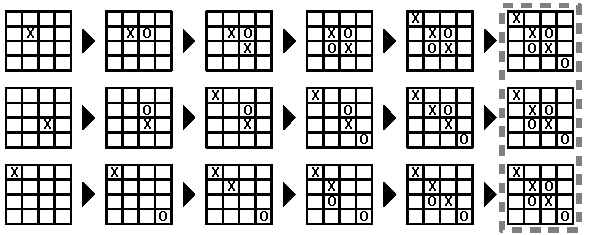
\includegraphics{inhalt/abbildungen/transitionen_tictactoe.pdf}
  \caption{Verschiedene Spielzugsequenzen enden im selben Spielzustand.}
  \label{fig:transitionen_tictactoe}
\end{figure} 

Übergänge innerhalb des Suchbaums verursachen Redundanzen. Für jede dieser Redundanzen wird eine erneute Suche durchgeführt, falls diese nicht durch Alpha-Beta-Kürzung abgeschnitten werden. Sollten diese Übergänge vermieden werden können, dann würde sich die Rechenzeit der Suchverfahren weiter verringern, weil weniger Spielzustände durchsucht bzw. expandiert werden müssen. Wie können wir Spielzustände in einer Übergangstabelle abspeichern? \\

\myparagraph{Zobrist Hash}
Wenn ein Computerprogramm einen Gegenstand in einer großen Tabelle speichert, muss die Tabelle zwangsläufig durchsucht werden, um den Gegenstand wiederzuverwenden bzw. zu referenzieren. Dies gilt solange, bis eine Tabellendresse aus dem Gegenstand selbst, in systematischer weise, berechnet werden kann. Eine Funktion die Gegenstände in Adressen umwandelt ist ein Hash-Algorithmus, und die daraus resultierende Tabelle ist eine Hashtabelle \cite[3]{Zobrist}. \\

\begin{figure}[!htbp]
  \centering
  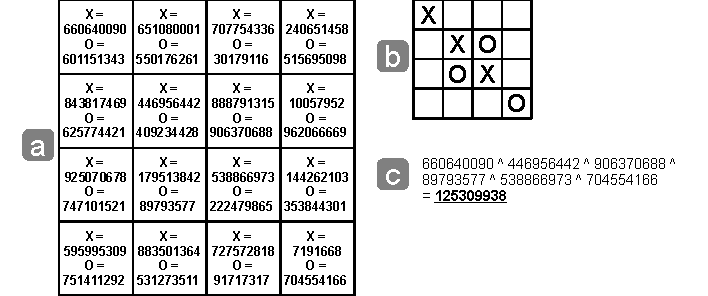
\includegraphics[scale = 1.3]{inhalt/abbildungen/zobrist_hash_tictactoe.pdf}
  \caption{Zobrist Hashing von Spielzuständen.}
  \label{fig:zobrist_hash_tictactoe}
\end{figure} 


In Abbildung \ref{fig:zobrist_hash_tictactoe} wird das Zobrist Hash Verfahrens auf den redundanten Spielzustand aus Abbildung \ref{fig:transitionen_tictactoe} angewendet. (\ref{fig:zobrist_hash_tictactoe} a) Wir weisen jedem Spielfeld zwei zufällige ganzzahlige Werte zu im Bereich von 0 bis maximal $1 \times 10^{9}$. Einen zufälligen Wert für den Kreuzspielstein an dieser Position und einen für den Kreisspielstein. Das 4x4 Tic Tac Toe Spielbrett sollte insgesamt 32 verschiedene Werte erhalten. (\ref{fig:zobrist_hash_tictactoe} b) Dieser Spielzustand soll in einen Zobrist-Hash umgewandelt werden. \\

(\ref{fig:zobrist_hash_tictactoe} c) Der Zobrist-Hash berechnet sich wie folgt, ist die aktuelle Position mit einem Kreuzspielstein oder einem Kreisspielstein besetzt, dann wähle den entsprechenden Wert aus (\ref{fig:zobrist_hash_tictactoe} a). Dies wiederhole für jedes besetzte Spielfeld. Auf den bereits ermittelten Wert und den hinzukommenden Wert wird ein exklusives bitweises Oder (XOR) angewendet. In Python ist das Zeichen für die Funktion des exklusiven bitweisen Oder ein Zirkumflex (siehe Operatoren in der Berechnung \ref{fig:zobrist_hash_tictactoe} c). Das Ergebnis ist eine Adresse die exakt den Spielzustand (\ref{fig:zobrist_hash_tictactoe} b) referenziert. \\

Spielzustände die gerade expandiert werden, können in die Übergangstabelle eingetragen werden, sollten diese nicht bereits in der Tabelle vorhanden sein. Ist dieser Spielzustand bereits in der Tabelle vorhanden, dann können die vorgeschlagenen besten Halbzüge aus der Tabelle ausgelesen und angewendet werden. \\

\subsection{Heuristik}
\label{subsec:Heuristik}
Eine Heuristik oder Bewertungsfunktion berechnet einen Nutzwert für einen gegebenen Spielzustand. Dieser Nutzwert gibt an, wie "wertvoll" diese Spielsituation hinsichtlich eines Sieges ist, sprich sie gibt an ob der Spieler in diesem Spielzustand eher gewinnen oder verlieren könnte. Trotz aller Optimierungen des Minimax Verfahrens (Alpha-Beta, Zugsortierung, Vermeidung von Redundanzen) wäre die Rechenzeit, für den zu durchsuchenden Baum, immer noch enorm hoch. Reale Zeitbeschränkungen z.B. bei Schach Spielen erlauben ein überaus langes Berechnen ohnehin nicht. Die Lösung ist das verwenden einer Heuristik. Der Kompromiss bei einer Heuristik ist: das Ergebnis wird geschätzt und ist nicht mehr sicher, aber die Suche kann nach einem Zeitkriterium abgebrochen werden und die beste bisher gefundene Lösung wird zurückgegeben. Sollte die Bewertungsfunktion für einen Spielzustand z.B. einen sehr hohen Wert berechnen, dann besagt dieser, der Spieler der diesen Spielzustand erreicht wird wahrscheinlich gewinnen. \\

Die Qualität einer Heuristik ist ausschlaggebend für die Spielerischen Fähigkeiten eines Programms. Ein Programm welches, durch eine schlechte Stellungsbewertung (Heuristik) einen fatalen Spielzug des Gegners übersieht oder ignoriert, würde gegen ein Programm verlieren, welches diese Stellungen (Spielzustände) erkennt und ausnutzt bzw. entsprechend verhindert. Eine Bewertungsfunktion B(s) für ein Schachspiel enthält folgende Elemente, wobei s der Parameter für den Spielzustand ist\cite[119]{Ertel}: \\

B(s) = $a_1$ x Material +  $a_2$ x Bauernstruktur + $a_3$ x Königssicherheit \\
\tab \tab + $a_4$ x Springer im Zentrum + $a_5$ x Läufer Diagonalabdeckung + ..., \\ 

das mit Abstand wichtigste Feature (Merkmal) "Material" nach der Formel \\

\tab \tab Material = Material(eigenes Team) - Material(Gegner) \\

Material(Team) = Anzahl Bauern(Team) x 100 + Anzahl Springer(Team) x 300 \\
\tab \tab \tab + Anzahl Läufer(Team) x 300 + Anzahl Türme(Team) x 500 \\
\tab \tab \tab + Anzahl Damen(Team) x 900 \\

Diese Schach Heuristik ist entstanden aus der Zusammenarbeit von Schachexperten und Wissensingenieuren. Die Schachexperten verfügen über Wissen und Erfahrungen bezüglich des Schachspiels, der Strategien, guter Zugstellungen und schlechter Zugstellungen. Der Wissensingenieur hat die meist sehr schwierige Aufgabe dieses Wissen in eine, für ein Programm, anwendbare Form zu bringen (vgl. \cite[118]{Ertel}). \\

Eine Heuristik ist stark Abhängig von ihrer Grundlage, d.h. eine Heuristik die für ein Schachspiel konzipiert wurde, berücksichtigt die Spielfiguren, das Spielfeld und die Spielregeln des Schachspiels. Wir können diese Heuristik nicht direkt auf Reversi oder Tic Tac Toe anwenden, weil eine Schach Heuristik nicht auf andere Spiele angewendet werden kann. Eine Reversi Heuristik kann z.B. auch nicht für das Spielen eines Tic Tac Toe Spiels verwendet werden. Es ist uns jedoch möglich das Konzept, sprich die Essenz der Heuristik Entwicklung, aus dieser Beispielheuristik für Schachspiele zu entnehmen und auf die Heuristik Entwicklung für Reversi und Tic Tac Toe anzuwenden. \\

Mehr zum Thema Heuristik Entwicklung in Kapitel \ref{cha:Modellierung und Entwurf} Modellierung und Entwurf, in diesem Kapitel werden wir ähnlich der gerade vorgestellten Heuristik, eigene Bewertungsfunktionen für Tic Tac Toe und Reversi entwerfen und in Kapitel \ref{cha:Implementierung} Implementierung, werden die modellierten Bewertungsfunktionen praktisch angewendet. \\

\myparagraph{Tic Tac Toe Heuristik}

\myparagraph{Reversi Heuristik}